% Boundary conditions of the one-element Hill runs ("isometric" and "free").
% Build: pdflatex hill_one_element_bcs.tex && pdftocairo -svg hill_one_element_bcs.pdf hill_one_element_bcs.svg
\documentclass[tikz,border=4pt]{standalone}
\usetikzlibrary{arrows.meta,patterns,calc}
\tikzset{
	edge/.style={thick},
	hidden/.style={thin,dashed,gray},
	fibre/.style={-{Latex[length=2.5mm]},very thick,blue!70!black},
	disp/.style={-{Latex[length=2mm]},thick,red!70!black},
	sym/.style={fill=gray!25,draw=none,opacity=0.85},
}
% unit cube in oblique projection: x right, y depth, z up
\newcommand{\cube}{%
	\coordinate (O) at (0,0); \coordinate (X) at (2,0); \coordinate (Y) at (0.9,0.6); \coordinate (Z) at (0,2);
	\coordinate (XY) at ($(X)+(Y)$); \coordinate (XZ) at ($(X)+(Z)$); \coordinate (YZ) at ($(Y)+(Z)$);
	\coordinate (XYZ) at ($(X)+(Y)+(Z)$);
}
\newcommand{\drawcube}{%
	\draw[hidden] (O) -- (Y) -- (XY) (Y) -- (YZ);
	\draw[edge] (O) -- (X) -- (XZ) -- (Z) -- cycle;
	\draw[edge] (X) -- (XY) -- (XYZ) -- (XZ) (Z) -- (YZ) -- (XYZ);
	\draw[fibre] ($(O)!0.5!(XZ)+(-0.45,0)$) -- ++(0.9,0) node[above=1pt] {$\mathbf f_0$};
}
\begin{document}
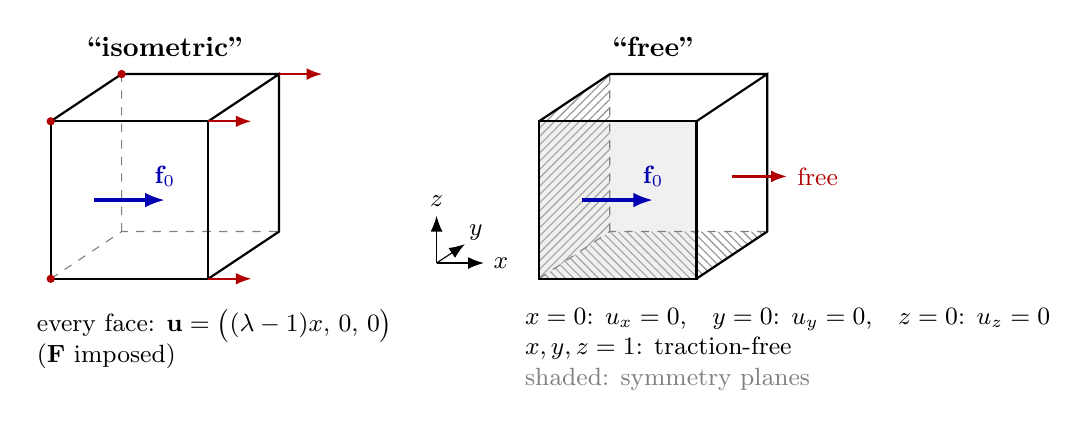
\begin{tikzpicture}[font=\small]
	% ---------------- isometric
	\begin{scope}
		\cube
		\drawcube
		\foreach \p in {XZ,X,XYZ} \draw[disp] (\p) -- ++(0.55,0);
		\foreach \p in {O,Z,YZ} \fill[red!70!black] (\p) circle (1.5pt);
		\node[font=\bfseries] at ($(O)!0.5!(X)+(0.45,2.95)$) {``isometric''};
		\node[align=left,anchor=north west] at (-0.3,-0.25)
			{every face: $\mathbf u = \big((\lambda-1)x,\,0,\,0\big)$\\ ($\mathbf F$ imposed)};
	\end{scope}
	% ---------------- free
	\begin{scope}[xshift=6.2cm]
		\cube
		% symmetry planes: x=0 (left), z=0 (bottom) hatched, y=0 (front) shaded
		\fill[sym,pattern=north east lines,pattern color=gray] (O) -- (Y) -- (YZ) -- (Z) -- cycle;
		\fill[sym,pattern=north west lines,pattern color=gray] (O) -- (X) -- (XY) -- (Y) -- cycle;
		\fill[gray!40,opacity=0.3] (O) -- (X) -- (XZ) -- (Z) -- cycle;
		\drawcube
		\draw[disp] ($(XZ)!0.5!(XY)$) -- ++(0.7,0) node[right] {free};
		% axes
		\draw[-{Latex[length=2mm]}] (-1.3,0.2) -- ++(0.6,0) node[right] {$x$};
		\draw[-{Latex[length=2mm]}] (-1.3,0.2) -- ++(0.36,0.24) node[above right=-2pt] {$y$};
		\draw[-{Latex[length=2mm]}] (-1.3,0.2) -- ++(0,0.6) node[above] {$z$};
		\node[font=\bfseries] at ($(O)!0.5!(X)+(0.45,2.95)$) {``free''};
		\node[align=left,anchor=north west] at (-0.3,-0.25)
			{$x = 0$: $u_x = 0$,\quad $y = 0$: $u_y = 0$,\quad $z = 0$: $u_z = 0$\\
			 $x, y, z = 1$: traction-free\\
			 {\color{gray}shaded: symmetry planes}};
	\end{scope}
\end{tikzpicture}
\end{document}
